\begin{figure}[htp]
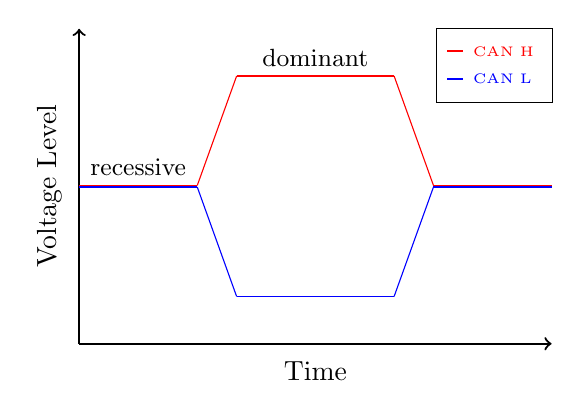
\begin{tikzpicture}
	%Draw axis
	\draw[thick,->] (0,0) -- coordinate (x axis mid) (6,0);
	\draw[thick,->] (0,0) -- coordinate (y axis mid) (0,4);
	%Draw axis label
	\node[below=0.1cm] at (x axis mid) {Time};
	\node[rotate=90, above=0.1cm] at (y axis mid) {Voltage Level};
	%Draw legend
	\matrix [draw,below left] at (current bounding box.north east) {
  		\draw[thick, red]  (0,0) -- (0.2,0) {} node[right]{\tiny CAN H}; \\
  		\draw[thick, blue] (0,0) -- (0.2,0){} node[right]{\tiny CAN L}; \\
	};

	%Draw CAN H
	\draw[red] (0,2.01)   -- (1.5,2.01) node[black, midway, above]{\small recessive};
	\draw[red] (1.5,2.01) -- (2,3.4);
	\draw[red] (2,3.4)    -- (4,3.4)    node[black, midway, above]{\small dominant};
	\draw[red] (4,3.4)    -- (4.5,2.01);
	\draw[red] (4.5,2.01) -- (6,2.01);
	%Draw CAN L
	\draw[blue] (0,1.99) -- (1.5,1.99);
	\draw[blue] (1.5,1.99) -- (2,0.6);
	\draw[blue] (2,0.6)    -- (4,0.6);
	\draw[blue] (4,0.6)    -- (4.5,1.99);
	\draw[blue] (4.5,1.99) -- (6,1.99);

	%
\end{tikzpicture}
\caption{CAN Physical Bit Transmission}
\label{fig:can_level}
\end{figure}